\chapter{}

Cauchy--Frobenius--Burnside's theorem is useful to
find characters. 

\begin{proposition}
    Let $G$ be 2-transitive on $X$ with character $\chi(g)=|\Fix(g)|$.
    Then $\chi-\chi_1$ is irreducible. 
\end{proposition}

\begin{proof}
    In particular, $G$ is transitive on $X$. 
    Since the trivial character $\chi_1$ is irreducible, $\langle\chi_1,\chi_1\rangle=1$. 
    By Cauchy--Frobenius--Burnside's, the rank of $G$ on $X$ is  
    \begin{gather*}
        2=\frac{1}{|G|}\sum_{g\in G}|\Fix(g)|^2=\langle \chi,\chi\rangle.
   \end{gather*}
   Thus $\langle \chi-\chi_1,\chi-\chi_1\rangle=\langle\chi,\chi\rangle-1-1+1=1$.
\end{proof}

\begin{example}
    The symmetric group $\Sym_n$ is 2-transitive on $\{1,\dots,n\}$. The
    alternating group $\Alt_n$ is 2-transitive on $\{1,\dots,n\}$ if 
    $n\geq4$. These groups then have an irreducible character $\chi$ 
    given by $\chi(g)=|\Fix(g)|-1$.
\end{example}

\begin{example}
    Let $p$ be a prime number and let $q=p^{m}$. Let $V$ 
    be the vector space of dimension $m$ 
    over the finite field of $q$ elements. 
    The group $G=\GL_2(q)$ acts 2-transitively on the set $X$ of
    one-dimensional subspaces of $V$. In fact, 
    if $\langle v\rangle\ne\langle v_1\rangle$ and $\langle w\rangle\ne\langle w_1\rangle$, 
    then $\{v,v_1\}$ and $\{w,w_1\}$ are bases of $V$. 
    The matrix $g$ that corresponds to the linear map 
    $v\mapsto w$, $v_1\mapsto w_1$, is invertible. Thus $g\in\GL_2(q)$. 
    The previous proposition produces the irreducible character
    $\chi(g)=|\Fix(g)|-1$. 
\end{example}

Now a combinatorial application:

\begin{example}
    In how many ways can we color (in black and white) the vertices of a square? 
    We will count colorings up to symmetric. This means that, for example, 
    the colorings 
    \begin{equation}
    \label{eq:orbita}
    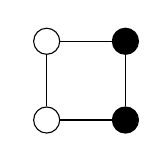
\begin{tikzpicture}
        \node[shape=circle,draw=black,fill=black] (A) at (1,0){};
        \node[shape=circle,draw=black,fill=black] (B) at (1,1){};
        \node[shape=circle,draw=black] (C) at (0,1){}; 
        \node[shape=circle,draw=black] (D) at (0,0){};
        \path [-](A) edge node[left]{} (B);
        \path [-](B) edge node[left]{} (C);
        \path [-](C) edge node[left]{} (D);
        \path [-](D) edge node[left]{} (A);
    \end{tikzpicture}
    \qquad
    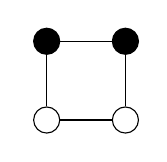
\begin{tikzpicture}
        \node[shape=circle,draw=black] (A) at (1,0) {};
        \node[shape=circle,draw=black,fill=black] (B) at (1,1) {};
        \node[shape=circle,draw=black,fill=black] (C) at (0,1) {};
        \node[shape=circle,draw=black] (D) at (0,0) {};
        \path [-](A) edge node[left]{} (B);
        \path [-](B) edge node[left]{} (C);
        \path [-](C) edge node[left]{} (D);
        \path [-](D) edge node[left]{} (A);
    \end{tikzpicture}
    \qquad
    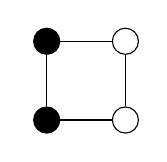
\begin{tikzpicture}
        \node[shape=circle,draw=black] (A) at (1,0) {};
        \node[shape=circle,draw=black] (B) at (1,1) {};
        \node[shape=circle,draw=black,fill=black] (C) at (0,1) {};
        \node[shape=circle,draw=black,fill=black] (D) at (0,0) {};
        \path [-](A) edge node[left]{} (B);
        \path [-](B) edge node[left]{} (C);
        \path [-](C) edge node[left]{} (D);
        \path [-](D) edge node[left]{} (A);
    \end{tikzpicture}
    \qquad
    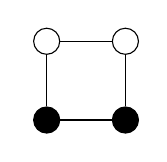
\begin{tikzpicture}
        \node[shape=circle,draw=black,fill=black] (A) at (1,0) {};
        \node[shape=circle,draw=black] (B) at (1,1) {};
        \node[shape=circle,draw=black] (C) at (0,1) {};
        \node[shape=circle,draw=black,fill=black] (D) at (0,0) {};
        \path [-](A) edge node[left]{} (B);
        \path [-](B) edge node[left]{} (C);
        \path [-](C) edge node[left]{} (D);
        \path [-](D) edge node[left]{} (A);
    \end{tikzpicture}
\end{equation}
will be considered as equivalent. Let $G=\langle g\rangle$ the cyclic 
group of order four. Let $X$ be 
the set of colorings of the square. Then 
$|X|=16$. 

Let $G$ acts on $X$ by anti-clockwise rotations  
of 90\textdegree. All the colorings of~\eqref{eq:orbita} belong to the same orbit. 
Another orbit of $X$ is
\[
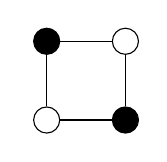
\begin{tikzpicture}
    \node[shape=circle,draw=black,fill=black] (A) at (1,0) {};
    \node[shape=circle,draw=black] (B) at (1,1) {};
    \node[shape=circle,draw=black,fill=black] (C) at (0,1) {};
    \node[shape=circle,draw=black] (D) at (0,0) {};
    \path [-](A) edge node[left]{} (B);
    \path [-](B) edge node[left]{} (C);
    \path [-](C) edge node[left]{} (D);
    \path [-](D) edge node[left]{} (A);
\end{tikzpicture}
\qquad
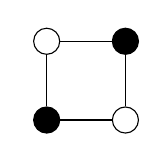
\begin{tikzpicture}
    \node[shape=circle,draw=black] (A) at (1,0) {};
    \node[shape=circle,draw=black,fill=black] (B) at (1,1) {};
    \node[shape=circle,draw=black] (C) at (0,1) {};
    \node[shape=circle,draw=black,fill=black] (D) at (0,0) {};
    \path [-](A) edge node[left]{} (B);
    \path [-](B) edge node[left]{} (C);
    \path [-](C) edge node[left]{} (D);
    \path [-](D) edge node[left]{} (A);
\end{tikzpicture}
\]

Cauchy--Frobenius--Burnside's theorem states that
there are  
\[
\frac{1}{|G|}\sum_{x\in G}|\Fix(x)|
\]
orbits. 

For each $x\in G=\{1,g,g^2,g^3\}$ we compute $\Fix(x)$. The identity fixes 
the 16 elements of $X$, both 
$g$ and  $g^3$ fix only two elements of $X$ and 
$g^2$ fixes four elements of $X$. For example, 
the elements of $X$ fixed by $g^2$ are 
\[
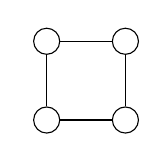
\begin{tikzpicture}
    \node[shape=circle,draw=black] (A) at (1,0){};
    \node[shape=circle,draw=black] (B) at (1,1){};
    \node[shape=circle,draw=black] (C) at (0,1){}; 
    \node[shape=circle,draw=black] (D) at (0,0){};
    \path [-](A) edge node[left]{} (B);
    \path [-](B) edge node[left]{} (C);
    \path [-](C) edge node[left]{} (D);
    \path [-](D) edge node[left]{} (A);
\end{tikzpicture}
\qquad
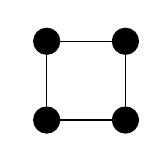
\begin{tikzpicture}
    \node[shape=circle,draw=black,fill=black] (A) at (1,0) {};
    \node[shape=circle,draw=black,fill=black] (B) at (1,1) {};
    \node[shape=circle,draw=black,fill=black] (C) at (0,1) {};
    \node[shape=circle,draw=black,fill=black] (D) at (0,0) {};
    \path [-](A) edge node[left]{} (B);
    \path [-](B) edge node[left]{} (C);
    \path [-](C) edge node[left]{} (D);
    \path [-](D) edge node[left]{} (A);
\end{tikzpicture}
\qquad
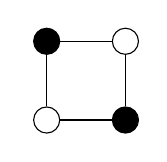
\begin{tikzpicture}
    \node[shape=circle,draw=black,fill=black] (A) at (1,0) {};
    \node[shape=circle,draw=black] (B) at (1,1) {};
    \node[shape=circle,draw=black,fill=black] (C) at (0,1) {};
    \node[shape=circle,draw=black] (D) at (0,0) {};
    \path [-](A) edge node[left]{} (B);
    \path [-](B) edge node[left]{} (C);
    \path [-](C) edge node[left]{} (D);
    \path [-](D) edge node[left]{} (A);
\end{tikzpicture}
\qquad
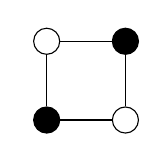
\begin{tikzpicture}
    \node[shape=circle,draw=black] (A) at (1,0) {};
    \node[shape=circle,draw=black,fill=black] (B) at (1,1) {};
    \node[shape=circle,draw=black] (C) at (0,1) {};
    \node[shape=circle,draw=black,fill=black] (D) at (0,0) {};
    \path [-](A) edge node[left]{} (B);
    \path [-](B) edge node[left]{} (C);
    \path [-](C) edge node[left]{} (D);
    \path [-](D) edge node[left]{} (A);
\end{tikzpicture}
\]
Thus $X$ is union of  
\[
\frac{1}{|G|}\sum_{x\in G}|\Fix(x)|=\frac{1}{4}(16+2+4+2)=6
\]
orbits. 
\end{example}

\begin{exercise}
    In how many ways (up to symmetry) can you
    arrange eight non-attacking rooks on a chessboard? Symmetries 
    are given by the dihedral group $\D_4$ of eight elements.
\end{exercise}

For a finite group $G$ let $\cp(G)$ be the probability 
that two random elements of $G$ commute. 
As an application of Cauchy--Frobenius--Burnside's theorem we
prove that 
$\cp(G)=k/|G|$, where $k$ is the number of conjugacy classes
of $G$.

\begin{theorem}
\index{Theorem!5/8}
\index{Erd\"os--Turan's theorem}
    If $G$ is a non-abelian finite group, then $\cp(G)\leq5/8$.
\end{theorem}

\begin{proof}
    Let $C=\{(x,y)\in G\times G:xy=yx\}$. We claim that  
    \[
    \cp(G)=\frac{|C|}{|G|^2}=\frac{k}{|G|}.
    \]
    In fact, let $G$ act on $G$ by conjugation. 
    By Cauchy--Frobenius--Burnside's theorem, 
    \[
    k=\frac{1}{|G|}\sum_{g\in G}|\Fix(g)|=\frac{1}{|G|}\sum_{g\in G}|C_G(g)|=\frac{|C|}{|G|},
    \]
    as $\Fix(g)=\{x\in G:gxg^{-1}=x\}=C_G(g)$ and $\sum_{g\in G}|C_G(g)|=|C|$. 

    We now claim that $k/|G|\leq 5/8$ if $G$ is non-abelian.
    
    Let $y_1,\dots,y_m$ the representatives of conjugacy classes of $G$ 
    of size $\geq2$. By the class equation, 
    \[
    |G|=|Z(G)|+\sum_{i=1}^m(G:C_G(y_i))\geq |Z(G)|+2m.
    \]
    Thus $m\leq(1/2)(|G|-|Z(G)|)$ and hence 
    \[
    k=|Z(G)|+m\leq |Z(G)|+\frac12(|G|-|Z(G)|)=\frac12(|Z(G)|+|G|).
    \]
    Since $G$ is non-abelian, $G/Z(G)$ is not cyclic. In particular, 
    $(G:Z(G))\geq4$. Therefore
    \[
    k\leq\frac12(|Z(G)|+|G|)\leq\frac12\left(\frac14+1\right)|G|,
    \]
    that is $k/|G|\leq 5/8$. 
\end{proof}

\begin{exercise}
    Prove that $\cp(Q_8)=5/8$. 
\end{exercise}

\begin{exercise}
    Let $G$ be a finite non-abelian group and $p$ be the smallest prime number
    dividing $|G|$. Prove that $\cp(G)\leq (p^2+p-1)/p^3$. Moreover, 
    the equality holds if and only if $(G:Z(G))=p^2$. 
\end{exercise}

\begin{exercise}
    Let $G$ be a finite group and $H$ be a subgroup of $G$.
    \begin{enumerate}
        \item $\cp(G)\leq\cp(H)$.
        \item If $H$ is normal in $G$, then $\cp(G)\leq\cp(G/H)\cp(H)$.
    \end{enumerate}
\end{exercise}

Degrees of irreducible characters give a lower bound:

\begin{proposition}
If $G$ is a finite group, then
\[
\cp(G)\geq\left(\frac{\sum_{\chi\in\Irr(G)}\chi(1)}{|G|}\right)^2.
\]
\end{proposition}

\begin{proof}
    Let $k$ be the number of conjugacy classes of $G$.
    By Cauchy--Schwarz's inequality, 
    \begin{align*}
        \left(\sum_{\chi\in\Irr(G)}\chi(1)\right)^2
        &\leq\left(\sum_{\chi\in\Irr(G)}\chi(1)^2\right)\left(\sum_{\chi\in\Irr(G)}1\right)^2
        =\left(\sum_{\chi\in\Irr(G)}\chi(1)^2\right)k=|G|k.
    \end{align*}
    From this the claim follows.
\end{proof}

\begin{theorem}[Dixon]
    \index{Dixon's theorem}
    If $G$ is a finite simple group, then $\cp(G)\leq1/12$.
\end{theorem}

The theorem appeared in 1970, as a problem in 
volume 13 of the \emph{Canadian Math. Bulletin}. The solution
appeared in 1973. 

\begin{exercise}
    Prove that $\cp(\Alt_5)=1/12$. 
\end{exercise}

The alternating group $\Alt_5$ is important in this setting:

\begin{theorem}[Guralnick--Robinson]
    \index{Guralnick--Robinson's theorem}
    If $G$ is a finite non-solvable group such that $\cp(G)>3/40$, then
    $G\simeq\Alt_5\times T$ for some abelian group 
    $T$ and $\cp(G)=1/12$. 
\end{theorem}

The proof appears in~\cite{MR2228209}.

Results on probability of commuting elements generalize in other directions. 
In~\cite{MR230809,MR276325,MR313378,MR369512}, 
Thompson proved the following result:

\begin{theorem}[Thompson]
\index{Thompson's theorem}
    If $G$ is a finite group such that 
    every pair of elements of $G$ generate
    a solvable group, then $G$ is solvable. 
\end{theorem}

The proof uses the classification of finite simple groups (CFSG). A simpler
proof independent of the CFSG appears in~\cite{MR1346207}.

There is a probabilistic version of Thompson's theorem:

\begin{theorem}[Guralnick--Wilson]
    \index{Guralnick--Wilson's theorem}
    Let $G$ be a finite group.
    \begin{enumerate}
        \item If the probability that two random elements of $G$ 
        generate a solvable group is $>11/30$, then $G$ is solvable. 
        \item If the probability that two random elements of $G$ 
        generate a nilpotent group is $>1/2$, then $G$ is nilpotent.
        \item If the probability that two random elements of $G$ 
        generate a group of odd order is $>11/30$, then $G$ has odd order.
    \end{enumerate}
\end{theorem}

The proof uses the CFSG and appears in~\cite{MR1770615}.



Nos basaremos en~\cite{MR1997347} y veremos otras aplicaciones del teorema de Cauchy--Frobenius--Burnside. 

\begin{theorem}[Jordan]
\index{Teorema!de Jordan}
Sea $G$ un grupo finito no trivial. Si $G$ actúa transitivamente en un conjunto finito $X$ y $|X|>1$, entonces
existe $g\in G$ sin puntos fijos. 
\end{theorem}

\begin{proof}
El teorema de Cauchy--Frobenius--Burnside implica que
\[
1=\frac{1}{|G|}\sum_{g\in G}|\Fix(g)|=\frac{1}{|G|}\left(|X|+\sum_{g\ne 1}|\Fix(g)|\right).
\]
Si todo $g\in G\setminus\{1\}$ contiene al menos un punto fijo, entonces
\[
1=\frac{1}{|G|}\left(|X|+\sum_{g\ne 1}|\Fix(g)|\right)\geq \frac{1}{|G|}(|X|+|G|-1)=1+\frac{|X|-1}{|G|}
\]
y luego $|X|\leq1$, una contradicción. 
\end{proof}

\begin{corollary}
Sea $G$ un grupo finito y $H$ un subgrupo propio de $G$. Entonces $G\ne\cup_{g\in G}gHg^{-1}$.
\end{corollary}

\begin{proof}
El grupo $G$ actúa transitivamente en $X=G/H$ por multiplicación a izquierda. 
El estabilizador de $xH$ es 
\[
G_{xH}=\{g\in G:gxH=xH\}=xHx^{-1}.
\]
Como $H\ne G$, entonces $|X|=|G/H|>1$. El teorema de Jordan implica entonces que existe $g\in G$ sin puntos fijos, es decir
que existe $g\in G$ tal que $g\not\in\cup_{x\in G}xHx^{-1}$. 
\end{proof}

Sea $G$ un grupo finito. Diremos que dos clases de conjugación $C$ y $D$ \textbf{conmutan} si existen 
$c\in C$ y $d\in D$ tales que $[c,d]=1$. 
Observemos que $C$ y $D$ conmutan si y sólo si para todo $c\in C$ existe $d\in D$ tal que $[c,d]=1$. 

\begin{corollary}[Wildon]
\index{Teorema!de Wildon}
    Sea $G$ un grupo finito y sea $C$ una clase de conjugación de $G$. Entonces
    $|C|=1$ si y sólo si $C$ conmuta con cualquier clase de conjugación de $G$. 
\end{corollary}
    
\begin{proof}
    Si $C=\{c\}$, entonces $c\in Z(G)$ y luego $C$ conmuta con cualquier clase de conjugación de $G$. Recíprocamente, supongamos que 
    $C$ conmuta con cualquier clase de conjugación de $G$. Si $c\in C$ y $H=C_G(c)$, entonces $H\cap D\ne\emptyset$ para toda
    clase de conjugación $D$. Afirmamos que entonces $G=\cup_{g\in G}gHg^{-1}$. En efecto, sea $x\in G$. Entonces $x\in D$ 
    para alguna clase de conjugación $D$. 
    Sea 
    $h\in H\cap D$. Existe $y\in G$ tal que $h=yxy^{-1}$, es decir $x=y^{-1}hy\in \cup_{g\in G}gHg^{-1}$. Por el teorema de Jordan, 
    $H=G$. Luego $c$ es central, es decir $C=\{c\}$. 
\end{proof}

La clasificación de grupos simples finitos permite demostrar un teorema
similar al teorema de Jordan~\cite{MR636194}. 

\begin{theorem}[Fein--Kantor--Schacher]
\index{Teorema!de Fein--Kantor--Schacher}
Sea $G$ un grupo finito no trivial. Si $G$ actúa transitivamente en un conjunto finito $X$ y $|X|>1$, entonces
existe un primo $p$ y un elemento $g\in G$ sin puntos fijos cuyo orden es una potencia de $p$. 
%existe $g\in G$ de orden una potencia de $p$ sin puntos fijos. 
\end{theorem}

No veremos la demostración en este curso. 

\index{Desarreglos}
Supongamos que $G$ es un grupo finito que actúa fiel y transitivamente en un conjunto $X$,
digamos $G\leq\Sym_n$, donde $X=\{1,2,\dots,n\}$. Sea 
$G_0$ el conjunto de $g\in G$ sin puntos fijos, es decir $g(x)\ne x$ para todo $x\in X$. 
Tales permutaciones se conocen como \textbf{desarreglos}. 
Sea $c_0=|G_0|/|G|$. 

\begin{theorem}[Cameron--Cohen]
\index{Teorema!de Cameron--Cohen}
Si $G$ es un subgrupo de $\Sym_n$ que actúa transitivamente en $\{1,\dots,n\}$, entonces $c_0\geq\frac{1}{n}$.
\end{theorem}

\begin{proof}
Sea $X=\{1,\dots,n\}$. El rango de $G$ es, por definición, la cantidad de orbitales de $G$ en $X$. Luego 
el rango de $G$ es $\geq2$, pues $X\times X$ puede descomponerse como 
$X\times X=\Delta\cup\left((X\times X)\setminus\Delta\right)$. 
Sean $\chi(g)=|\Fix(g)|$ y $G_0=\{g\in G:\chi(g)=0\}$. Si $g\not\in G_0$, entonces $1\leq\chi(g)\leq n$. Como 
$(\chi(g)-1)(\chi(g)-n)\leq 0$,
se tiene que 
\[
\frac{1}{|G|}\sum_{g\in G\setminus G_0}(\chi(g)-1)(\chi(g)-n)\leq 0.
\]
Por un lado, 
\begin{align*}
\frac{1}{|G|}\sum_{g\in G}(\chi(g)&-1)(\chi(g)-n)\\
&=\frac{1}{|G|}\left\{\sum_{g\in G_0}+\sum_{g\in G\setminus G_0}\right\}(\chi(g)-1)(\chi(g)-n)\\
&\leq n\frac{|G_0|}{|G|}=nc_0.
\end{align*}
Por otro lado, como el rango de $G$ es $\geq2$, tenemos 
\begin{equation}
    \label{eq:CameronCohen}
    2-\frac{n+1}{|G|}\sum_{g\in G}\chi(g)+n\leq 
    \frac{1}{|G|}\sum_{g\in G}(\chi(g)-1)(\chi(g)-n)\leq nc_0.
\end{equation}
Por hipotesis, $G$ es transitivo en $X$. El teorema de Cauchy--Frobenius--Burnside implica entonces que 
$\sum_{g\in G}\chi(g)=|G|$. Se sigue que $2-(n+1)+n\leq nc_0$ y luego $1/n\leq c_0$. 
% Si $c_0=1/n$, entonces $G$ tiene rango dos (pues si el rango de $G$ es $>2$ entonces la fórmula~\eqref{eq:CameronCohen}
% implica que $1/n<c_0$). Además, por un lado, 
% \begin{align*}
% \frac{1}{|G|}\sum_{g\in G}(\chi(g)-1)(\chi(g)-n)&=\frac{1}{|G|}\sum_{g\in G}\chi(g)^2-\frac{n+1}{|G|}\sum_{g\in G}\chi(g)+n\\
% &=2-(n+1)+n=1.    
% \end{align*}
% Por otro lado, como $c_0=|G_0|/|G|=1/n$, 
% \begin{align*}
% \frac{1}{|G|}\sum_{g\in G}(\chi(g)-1)(\chi(g)-n)
% &=\frac{1}{|G|}\sum_{g\in G\setminus G_0}(\chi(g)-1)(\chi(g)-n)\\
% &=\frac{1}{|G|}\sum_{g\in G_0}(\chi(g)-1)(\chi(g)-n)\\
% &=\frac{1}{|G|}\sum_{g\in G\setminus G_0}(\chi(g)-1)(\chi(g)-n)+1.
% \end{align*}
% Luego $\frac{1}{|G|}\sum_{g\in G\setminus G_0}(\chi(g)-1)(\chi(g)-n)=0$ y entonces $(\chi(g)-1)(\chi(g)-n)$ para todo $g\in G\setminus G_0$.
\end{proof}

El teorema de Cameron--Cohen tiene una segunda parte: 
Si $n$ no es potencia de un primo, entonces $c_0>1/n$. 
Daremos la demostración en el capítulo~\ref{Frobenius}, donde 
estudiaremos grupos de Frobenius.  

La cota del teorema de Cameron--Cohen puede mejorarse si se utiliza la 
clasificación de grupos simples finitos~\cite{MR1484879}.  

\begin{theorem}[Guralnick--Wan]
\index{Teorema!de Guralnick--Wan}
Sea $G$ un grupo finito transitivo de grado $n\geq2$. Si $n$ no es potencia de un 
número primo 
y además $G\ne\Sym_n$ para $n\in\{2,4,5\}$, entonces $c_0\geq 2/n$.
\end{theorem}

La demostración utiliza la clasificación de grupos finitos 2-transitivos, que depende del 
la clasificación de grupos simples finitos.



